\documentclass{article}
\usepackage{graphicx}  % Required for \resizebox
\usepackage{booktabs}   % For better table formatting
\usepackage{pdflscape}  % For landscape pages

\begin{document}

\begin{table}[h]
    \centering
    \renewcommand{\arraystretch}{1.3}
    \resizebox{\textwidth}{!}{ % Resizes the table to fit the page width
    \begin{tabular}{|l|l|l|}
        \hline
        \textbf{RCC Relation} & \textbf{Filtering Step (MBR Approximation)} & \textbf{Refinement Step (Exact Check)} \\
        
        \hline
        \textbf{Disjoint (DC)} & \texttt{NOT ST\_Intersects(A.MBR, B.MBR)} & \texttt{ST\_Disjoint(A.geom, B.geom)} \\
        \hline
        \textbf{Externally Connected (EC)} & \texttt{ST\_Intersects(A.MBR, B.MBR)} & \texttt{ST\_Touches(A.geom, B.geom)} \\
        \hline
        \textbf{Partially Overlapping (PO)} & \texttt{ST\_Intersects(A.MBR, B.MBR)} & \texttt{ST\_Overlaps(A.geom, B.geom)} \\
        \hline
        \textbf{Equal (EQ)} & \texttt{ST\_Intersects(A.MBR, B.MBR)} & \texttt{ST\_Equals(A.geom, B.geom)} \\
        \hline
        \textbf{Tangential Proper Part (TPP)} & \texttt{ST\_Contains(B.MBR, A.MBR)} & \texttt{ST\_Contains(B.geom, A.geom) AND ST\_Touches(A.geom, B.geom)} \\
        \hline
        \textbf{Non-Tangential Proper Part (NTPP)} & \texttt{ST\_Contains(B.MBR, A.MBR)} & \texttt{ST\_Within(A.geom, B.geom)} \\ 
        \hline
    \end{tabular}}
    \caption{Filtering \& Refinement Steps for RCC Filters}
    \label{tab:rcc_filtering}
\end{table}

\begin{table}[h]
    \centering
    \renewcommand{\arraystretch}{1.3}
    \resizebox{\textwidth}{!}{
    \begin{tabular}{|l|p{0.6\textwidth}|}
        \hline
        \textbf{RCC Relation} & \textbf{Formal Definition} \\
        \hline
        \textbf{Disjoint (DC)} & $A \cap B = \emptyset$ \\
        \hline
        \textbf{Externally Connected (EC)} & $interior(A) \cap interior(B) = \emptyset \land boundary(A) \cap boundary(B) \neq \emptyset$ \\
        \hline
        \textbf{Partially Overlapping (PO)} & $interior(A) \cap interior(B) \neq \emptyset \land A \not\subseteq B \land B \not\subseteq A$ \\
        \hline
        \textbf{Equal (EQ)} & $A = B$ \\
        \hline
        \textbf{Tangential Proper Part (TPP)} & $A \subset B \land boundary(A) \cap boundary(B) \neq \emptyset$ \\
        \hline
        \textbf{Non-Tangential Proper Part (NTPP)} & $A \subset B \land boundary(A) \cap boundary(B) = \emptyset$ \\
        \hline
    \end{tabular}}
    \caption{Formal Definitions of RCC Relations}
    \label{tab:rcc_formal}
\end{table}

\begin{figure}[htbp]
    \centering
    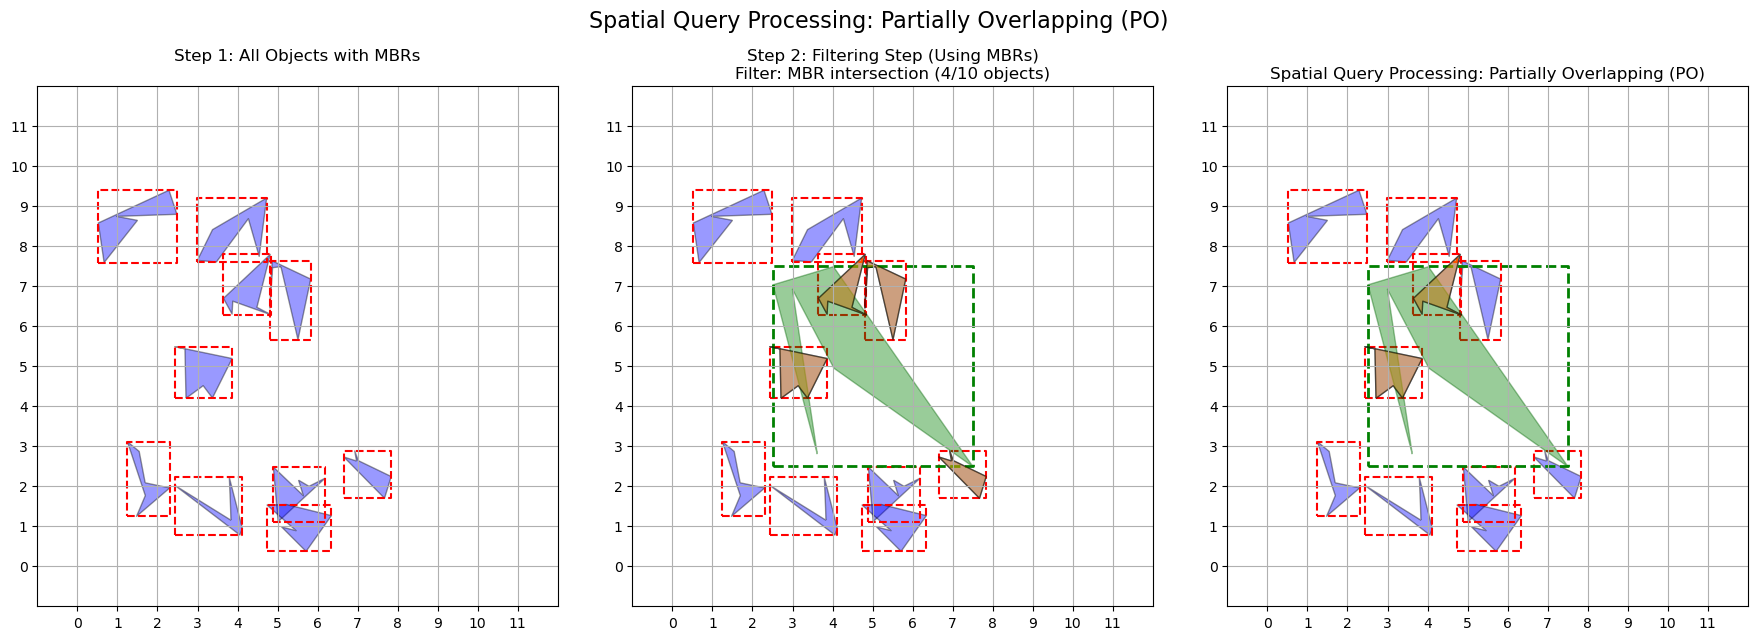
\includegraphics[width=1\linewidth]{figs/overlaps.png}
    \caption{Overlaps}
    \label{fig:MAE_MAPE_with_min_number_of_object}
\end{figure}

....


\begin{table}[h]
    \centering
    \renewcommand{\arraystretch}{1.3}
    \resizebox{\textwidth}{!}{ % Resizes the table to fit the page width
    \begin{tabular}{|l|l|l|}
        \hline
        \textbf{Distance Filter} & \textbf{Filtering Step (MBR Approximation)} & \textbf{Refinement Step (Exact Check)} \\
        \hline
        \textbf{Distance(A, B) $\leq$ d} & \texttt{ST\_DWithin(A.MBR, B.MBR, d)} & \texttt{ST\_DWithin(A.geom, B.geom, d)} \\
        \hline
        \textbf{Distance(A, B) $\geq$ d} & \texttt{NOT ST\_DWithin(A.MBR, B.MBR, d)} & \texttt{ST\_Distance(A.geom, B.geom) > d} \\
        \hline
        \textbf{k-Nearest Neighbors (KNN)} & \texttt{ORDER BY ST\_Distance(A.MBR, B.MBR) LIMIT k} & \texttt{ORDER BY ST\_Distance(A.geom, B.geom) LIMIT k} \\
        \hline
        \textbf{Farthest Neighbors (FNN)} & \texttt{ORDER BY ST\_Distance(A.MBR, B.MBR) DESC LIMIT k} & \texttt{ORDER BY ST\_Distance(A.geom, B.geom) DESC LIMIT k} \\
        \hline
        \textbf{Objects in Range [$d_1, d_2$]} & \texttt{ST\_DWithin(A.MBR, B.MBR, $d_2$) AND NOT ST\_DWithin(A.MBR, B.MBR, $d_1$)} & \texttt{$d_1 \leq$ ST\_Distance(A.geom, B.geom) $\leq d_2$} \\
        \hline
    \end{tabular}}
    \caption{Filtering \& Refinement Steps for Distance-Based Filters}
    \label{tab:distance_filtering}
\end{table}

\begin{table}[h]
    \centering
    \renewcommand{\arraystretch}{1.3}
    \resizebox{\textwidth}{!}{
    \begin{tabular}{|l|p{0.6\textwidth}|}
        \hline
        \textbf{Distance Filter} & \textbf{Formal Definition} \\
        \hline
        \textbf{Distance(A, B) $\leq$ d} & $\min\{dist(p,q) \mid p \in A, q \in B\} \leq d$ \\
        \hline
        \textbf{Distance(A, B) $\geq$ d} & $\min\{dist(p,q) \mid p \in A, q \in B\} \geq d$ \\
        \hline
        \textbf{k-Nearest Neighbors (KNN)} & For a query region $Q$, return set $S$ of $k$ objects where $\forall o \in S, \forall o' \not\in S: dist(Q,o) \leq dist(Q,o')$ \\
        \hline
        \textbf{Farthest Neighbors (FNN)} & For a query region $Q$, return set $S$ of $k$ objects where $\forall o \in S, \forall o' \not\in S: dist(Q,o) \geq dist(Q,o')$ \\
        \hline
        \textbf{Objects in Range [$d_1, d_2$]} & For a query region $Q$, return all objects $o$ where $d_1 \leq dist(Q,o) \leq d_2$ \\
        \hline
    \end{tabular}}
    \caption{Formal Definitions of Distance-Based Filters}
    \label{tab:distance_formal}
\end{table}


\subsection{Spatial Selectivity Estimation as a Regression Problem}

We formulate spatial selectivity estimation as a regression problem that focuses on the filtering step of spatial query processing. Our analysis of the RCC (Region Connection Calculus) relations, as shown in Table~\ref{tab:rcc_filtering}, demonstrates that all topological spatial relationships can be effectively filtered using just two fundamental spatial predicates: \textbf{Intersect} and \textbf{Contain}. These two operations form the foundation of spatial filtering:

\begin{itemize}
\item \textbf{Intersect} filters cover Disjoint (negated), Externally Connected, Partially Overlapping, and Equal relations
\item \textbf{Contain} filters cover Tangential Proper Part (TPP) and Non-Tangential Proper Part (NTPP) relations
\end{itemize}

Additionally, we extend our approach to include \textbf{Distance}-based filters, which support proximity queries beyond standard RCC relations. Since the filtering step determines which objects must be retrieved from spatial indexes before performing the more expensive refinement with exact geometries, accurate estimation of filtering selectivity is essential for query optimization.

Let $T$ represent a spatial dataset containing objects with associated MBRs. For a query clause $c$ with geometry $g$, we define:

\begin{itemize}
\item $MBR(c)$ denotes the Minimum Bounding Rectangle of geometry $g$, represented as $\langle x_{\min}, y_{\min}, x_{\max}, y_{\max} \rangle$
\item $act_{intersect}(c)$ represents the number of objects in $T$ whose MBRs intersect with $MBR(c)$
\item $act_{contain}(c)$ represents the number of objects in $T$ whose MBRs are contained within $MBR(c)$
\item $act_{distance}(c, d_1, d_2)$ represents the number of objects in $T$ whose MBRs are at a distance $d$ from $MBR(c)$ where $d_1 < d < d_2$
\end{itemize}

For training our regression models, we collect labeled clauses in the form:
\begin{align}
S_{intersect} &= \{\langle MBR(c): act_{intersect}(c) \rangle\} \\
S_{contain} &= \{\langle MBR(c): act_{contain}(c) \rangle\} \\
S_{distance} &= \{\langle MBR(c), d_1, d_2: act_{distance}(c, d_1, d_2) \rangle\}
\end{align}

\textbf{Problem:} Given these sets of labeled clauses, we aim to learn three regression models $M_{intersect}$, $M_{contain}$, and $M_{distance}$, such that for any clause $c$ on dataset $T$, each model produces an estimated selectivity close to the actual selectivity for its respective filter type:
\begin{align}
est_{intersect}(c) &\approx act_{intersect}(c) \\
est_{contain}(c) &\approx act_{contain}(c) \\
est_{distance}(c, d_1, d_2) &\approx act_{distance}(c, d_1, d_2)
\end{align}

Focusing on these core filter types allows us to efficiently estimate the cost of retrieving objects using spatial indexes. Accurate selectivity estimation directly impacts:
\begin{itemize}
\item Selection of efficient query execution plans
\item I/O cost estimation for retrieving objects from spatial indexes  
\item Optimal ordering of spatial join operations
\end{itemize}

For the distance-based filter, we incorporate additional features $d_1$ and $d_2$ to represent the minimum and maximum distance thresholds, extending our input feature vector from $\mathbb{R}^4$ to $\mathbb{R}^6$.
\subsection{Feature Engineering for Distance Filters}

For the distance-based filter estimation, the standard MBR representation $(x_{\min}, y_{\min}, x_{\max}, y_{\max})$ is augmented with distance parameters $(d_1, d_2)$. This creates a challenge as the input space dimensionality increases from 4 to 6 dimensions.

To effectively model this expanded problem, we consider several transformations of the input features:

\begin{equation}
\mathbf{z_i} = x_i \oplus \bigoplus_{k=1}^m \Phi_k(x_i)
\end{equation}

where $x_i = (x_{\min}, y_{\min}, x_{\max}, y_{\max}, d_1, d_2)$ and $\Phi_k$ represent feature transformations such as:
\begin{itemize}
\item MBR center coordinates: $(x_{center}, y_{center}) = ((x_{max} + x_{min})/2, (y_{max} + y_{min})/2)$
\item MBR dimensions: $width = (x_{max} - x_{min})$, $height = (y_{max} - y_{min})$
\item Area of the MBR: $area = (x_{max} - x_{min}) \cdot (y_{max} - y_{min})$
\item Normalized center coordinates: $norm_x = \frac{x_{center} - univ_{x_{min}}}{univ_{x_{max}} - univ_{x_{min}}}$, $norm_y = \frac{y_{center} - univ_{y_{min}}}{univ_{y_{max}} - univ_{y_{min}}}$
\item Distance range: $d_{range} = d_2 - d_1$
\item Distance ratio: $d_{ratio} = \frac{d_2}{max(d_1, \epsilon)}$, where $\epsilon$ is a small constant to avoid division by zero
% \item Area of the MBR: $(x_{\max} - x_{\min}) \cdot (y_{\max} - y_{\min})$
% \item Perimeter of the MBR: $2 \cdot ((x_{\max} - x_{\min}) + (y_{\max} - y_{\min}))$
% \item Distance range size: $(d_2 - d_1)$
% \item Area of expanded MBR with distance $d_2$: $(x_{\max} + d_2 - (x_{\min} - d_2)) \cdot (y_{\max} + d_2 - (y_{\min} - d_2))$
\end{itemize}

\begin{table}[h]
    \centering
    \caption{Feature Transformations for Spatial Filter Estimation}
    \label{tab:feature-transformations}
    \renewcommand{\arraystretch}{1.3}
    \begin{tabular}{|l|l|p{7cm}|}
        \hline
        \textbf{Feature Type} & \textbf{Notation} & \textbf{Definition} \\
        \hline
        \multicolumn{3}{|c|}{\textbf{MBR Basic Coordinates}} \\
        \hline
        Original MBR & $x_i$ & $(x_{\min}, y_{\min}, x_{\max}, y_{\max})$ \\
        \hline
        \multicolumn{3}{|c|}{\textbf{Derived Spatial Features}} \\
        \hline
        MBR Center & $(x_{center}, y_{center})$ & $((x_{\max} + x_{\min})/2, (y_{\max} + y_{\min})/2)$ \\
        \hline
        MBR Dimensions & $width, height$ & $width = (x_{\max} - x_{\min}), height = (y_{\max} - y_{\min})$ \\
        \hline
        MBR Area & $area$ & $(x_{\max} - x_{\min}) \cdot (y_{\max} - y_{\min})$ \\
        \hline
        Normalized Center & $norm_x, norm_y$ & $norm_x = \frac{x_{center} - univ_{x_{min}}}{univ_{x_{max}} - univ_{x_{min}}}$ \\
        & & $norm_y = \frac{y_{center} - univ_{y_{min}}}{univ_{y_{max}} - univ_{y_{min}}}$ \\
        \hline
        \multicolumn{3}{|c|}{\textbf{Distance Filter Features}} \\
        \hline
        Distance Parameters & $d_1, d_2$ & Minimum and maximum distance thresholds \\
        \hline
        Distance Range & $d_{range}$ & $d_2 - d_1$ \\
        \hline
        Distance Ratio & $d_{ratio}$ & $\frac{d_2}{max(d_1, \epsilon)}$, where $\epsilon$ is a small constant \\
        \hline
    \end{tabular}
\end{table}

\begin{table}
    \centering
    \begin{tabular}{|c|c|c|}
    \hline
       & \textbf{Transformation} & $d_k$ \\
    \hline
    $\Phi_1(x_i)$ & MBR center coordinates: $(x_{center}, y_{center}) = ((x_{max} + x_{min})/2, (y_{max} + y_{min})/2)$ & 2 \\
    \hline
    $\Phi_2(x_i)$ & MBR dimensions: $width = (x_{max} - x_{min})$, $height = (y_{max} - y_{min})$ & 2 \\
    \hline
    $\Phi_3(x_i)$ & MBR area: $area = (x_{max} - x_{min}) \cdot (y_{max} - y_{min})$ & 1 \\
    \hline
    $\Phi_4(x_i)$ & Normalized center coordinates: $norm_x = \frac{x_{center} - univ_{x_{min}}}{univ_{x_{max}} - univ_{x_{min}}}$, $norm_y = \frac{y_{center} - univ_{y_{min}}}{univ_{y_{max}} - univ_{y_{min}}}$ & 2 \\
    \hline
    $\Phi_5(x_i)$ & Distance range: $d_{range} = d_2 - d_1$ & 1 \\
    \hline
    $\Phi_6(x_i)$ & Distance ratio: $d_{ratio} = \frac{d_2}{max(d_1, \epsilon)}$ & 1 \\
    \hline
    \end{tabular}   
    \caption{Feature transformations $\Phi_k(.)$ and their associated dimensions.}
    \label{tab:phi}
\end{table}


These engineered features help the regression models better capture the relationship between MBR characteristics, distance thresholds, and the resulting selectivity.


\subsection{Specialization of Distance Filters}

The distance filter estimation framework, which takes parameters $MBR(c)$, $d_1$, and $d_2$, is designed as a general approach that can handle various distance-based predicates through appropriate parameter settings. This section demonstrates how common distance predicates can be expressed through this framework:

\begin{itemize}
\item \textbf{Distance(A, B) $<$ d}: This common "within distance" predicate can be expressed by setting $d_1 = 0$ and $d_2 = d$. This finds all objects whose MBRs are within distance $d$ of the query MBR:

\begin{align}
est_{distance}(c, 0, d) &\approx act_{distance}(c, 0, d) \\
&= |\{o \in T \mid dist(MBR(c), MBR(o)) < d\}|
\end{align}

\item \textbf{Distance(A, B) $>$ d}: The "beyond distance" predicate can be handled by setting $d_1 = d$ and $d_2 = \infty$, where $\infty$ can be represented either by the universe bounds or by estimating it as the total number of objects minus the count of objects with Distance(A, B) $<$ d:

\begin{align}
est_{distance}(c, d, \infty) &\approx act_{distance}(c, d, \infty) \\
&= |\{o \in T \mid dist(MBR(c), MBR(o)) > d\}| \\
&= |T| - |\{o \in T \mid dist(MBR(c), MBR(o)) \leq d\}|
\end{align}

\item \textbf{k-Nearest Neighbors (KNN)}: While this framework does not directly estimate KNN results, it can be used to estimate the number of objects within successive distance bands, which helps determine appropriate distance thresholds for KNN searches.

\item \textbf{Distance Band}: The framework directly estimates the number of objects that fall within a distance band $[d_1,d_2]$:

\begin{align}
est_{distance}(c, d_1, d_2) &\approx act_{distance}(c, d_1, d_2) \\
&= |\{o \in T \mid d_1 \leq dist(MBR(c), MBR(o)) \leq d_2\}|
\end{align}
\end{itemize}


....

\begin{landscape}
\begin{table}
\centering
\caption{Model Performance Metrics for Intersect Filter}
\label{tab:model-comparison-intersect}
\resizebox{\linewidth}{!}{
\begin{tabular}{l|cccccc|cccccc|cccccc|cccccc|cccccc}
\toprule
Dataset & Histogram & RTree & KNN & NN & RF & XGB & Histogram & RTree & KNN & NN & RF & XGB & Histogram & RTree & KNN & NN & RF & XGB & Histogram & RTree & KNN & NN & RF & XGB & Histogram & RTree & KNN & NN & RF & XGB \\
\midrule
& \multicolumn{6}{c|}{Build (s)} & \multicolumn{6}{c|}{Size (MB)} & \multicolumn{6}{c|}{Time (ms)} & \multicolumn{6}{c|}{MAE} & \multicolumn{6}{c}{MAPE (\%)} \\
\midrule
zcta5 & \textbf{$<$0.01} & 1.65 & $<$0.01 & 11.20 & 1.22 & 4.48 & \textbf{0.02} & 2.20 & 0.34 & 0.07 & 0.75 & 0.04 & 0.03 & \textbf{$<$0.01} & 0.05 & $<$0.01 & 0.06 & $<$0.01 & 101.21 & 445.12 & 216.08 & 298.38 & \textbf{98.29} & 163.40 & \textbf{30.78} & 235.70 & 99.19 & 112.74 & 112.59 & 81.53 \\
aerowaythingnodesorted & \textbf{$<$0.01} & 3.78 & $<$0.01 & 96.88 & 15.50 & 10.14 & \textbf{0.06} & 5.09 & 0.82 & 0.07 & 27.83 & 0.47 & 0.03 & \textbf{$<$0.01} & 0.35 & 0.03 & 0.19 & 0.01 & \textbf{168.50} & 722.70 & 348.01 & 720.35 & 252.63 & 216.57 & \textbf{172.07} & 1377.19 & 191.77 & 1594.09 & 462.65 & 312.13 \\
craftwaysorted & \textbf{$<$0.01} & 5.07 & $<$0.01 & 155.07 & 20.84 & 10.30 & 0.08 & 6.90 & 1.14 & \textbf{0.07} & 25.51 & 0.48 & 0.03 & \textbf{$<$0.01} & 0.24 & 0.04 & 0.15 & 0.01 & 203.83 & 1244.86 & 604.33 & 829.54 & 176.71 & \textbf{173.88} & \textbf{49.94} & 486.88 & 86.09 & 430.47 & 76.19 & 90.21 \\
arealm & \textbf{$<$0.01} & 5.97 & 0.01 & 208.51 & 17.67 & 10.65 & 0.10 & 8.34 & 1.33 & \textbf{0.07} & 11.07 & 0.46 & 0.03 & \textbf{$<$0.01} & 0.28 & 0.04 & 0.08 & 0.01 & 216.22 & 1642.61 & 604.19 & 960.31 & 170.85 & \textbf{159.03} & \textbf{35.25} & 931.34 & 341.68 & 479.30 & 61.69 & 53.65 \\
emergencythingwaysorted & 3.00 & 46.04 & \textbf{0.09} & 1073.72 & 45.80 & 16.32 & 0.62 & 51.57 & 8.69 & \textbf{0.25} & 31.63 & 0.56 & 0.05 & 0.02 & 0.61 & 0.11 & 0.02 & \textbf{$<$0.01} & 473.72 & 4587.46 & 2495.43 & 2231.63 & \textbf{467.79} & 752.17 & \textbf{38.86} & 1077.19 & 187.94 & 436.17 & 56.74 & 277.61 \\
historicthingwaysorted & 8.00 & 100.14 & \textbf{0.21} & 2193.16 & 124.15 & 21.51 & 1.37 & 114.02 & 19.24 & \textbf{0.23} & 65.66 & 0.56 & 0.09 & 0.02 & 0.60 & 0.11 & 0.02 & \textbf{$<$0.01} & \textbf{776.42} & 5735.42 & 3615.25 & 2541.19 & 827.39 & 1259.62 & \textbf{24.11} & 352.10 & 115.41 & 353.37 & 36.88 & 258.62 \\
aerowaythingwaysorted & 10.00 & 96.26 & \textbf{0.21} & 1437.41 & 125.42 & 22.42 & 1.40 & 116.49 & 19.85 & \textbf{0.25} & 83.86 & 0.58 & 0.09 & 0.02 & 0.68 & 0.13 & 0.02 & \textbf{$<$0.01} & \textbf{800.09} & 3645.65 & 3075.73 & 2768.11 & 1260.26 & 2154.97 & \textbf{48.06} & 485.98 & 197.90 & 507.42 & 78.47 & 500.72 \\
areawater & 13.00 & 128.52 & \textbf{0.26} & 2416.90 & 166.69 & 22.67 & 1.74 & 146.79 & 23.98 & \textbf{0.24} & 23.76 & 0.55 & 0.10 & 0.01 & 0.63 & 0.20 & $<$0.01 & \textbf{$<$0.01} & 870.11 & 5168.13 & 4802.73 & 2002.21 & \textbf{839.96} & 1180.20 & 33.53 & 1733.05 & 331.48 & 324.95 & \textbf{17.91} & 177.09 \\
yago2 & 4970.00 & 224.82 & \textbf{0.63} & 2064.22 & 365.49 & 39.87 & 2.00 & 294.96 & 48.84 & \textbf{0.22} & 321.37 & 0.59 & 0.12 & 0.05 & 0.93 & 0.09 & 0.04 & \textbf{$<$0.01} & 42.36K & 19.19K & 5264.34 & 6098.01 & \textbf{2415.38} & 5774.85 & 61.78 & 73.86 & 21.98 & 293.02 & \textbf{3.10} & 313.25 \\
cyclewaythingwaysorted & 19.00 & 327.70 & \textbf{0.77} & 5087.37 & 470.00 & 40.39 & 2.00 & 336.84 & 56.51 & \textbf{0.24} & 153.99 & 0.58 & 0.11 & 0.03 & 0.54 & 0.10 & 0.02 & \textbf{$<$0.01} & 1839.62 & 9123.38 & 7902.84 & 8117.05 & \textbf{1630.39} & 4174.72 & 45.20 & 1060.91 & 303.49 & 1657.30 & \textbf{35.26} & 923.23 \\
powerthingnodesorted & 67.00 & 823.39 & \textbf{2.11} & 5611.14 & 1083.75 & 74.60 & 2.00 & 686.41 & 112.28 & \textbf{0.23} & 402.83 & 0.59 & 0.12 & 0.05 & 0.83 & 0.11 & 0.03 & \textbf{$<$0.01} & 3757.83 & 7986.18 & 10.25K & 13.30K & \textbf{3626.45} & 10.02K & 74.79 & 3149.50 & 777.38 & 8244.39 & \textbf{70.87} & 6142.80 \\
powerthingwaysorted & 71.00 & 3553.07 & \textbf{3.31} & 4947.33 & 1465.60 & 99.79 & 2.00 & 874.00 & 148.57 & \textbf{0.23} & 526.77 & 0.59 & 0.12 & 0.06 & 0.59 & 0.08 & 0.03 & \textbf{$<$0.01} & 4957.00 & 8848.55 & 12.45K & 14.69K & \textbf{4036.76} & 12.53K & 51.36 & 843.06 & 245.55 & 4221.51 & \textbf{42.74} & 2463.70 \\
barrierthingwaysorted & 89.00 & 1390.41 & \textbf{5.96} & 6326.01 & 2535.52 & 87.23 & 2.00 & 1456.02 & 244.92 & \textbf{0.24} & 910.45 & 0.30 & 0.12 & 0.08 & 0.93 & 0.09 & 0.04 & \textbf{$<$0.01} & 8490.12 & 16.56K & 23.39K & 23.24K & \textbf{4564.90} & 20.81K & 61.64 & 376.86 & 245.17 & 4279.45 & \textbf{35.92} & 2018.65 \\
leisurewaysorted & 96.00 & 3285.01 & \textbf{6.89} & 7940.58 & 3002.09 & 182.14 & 2.00 & 1866.90 & 275.34 & \textbf{0.24} & 958.73 & 0.59 & 0.12 & 0.09 & 0.56 & 0.08 & 0.04 & \textbf{$<$0.01} & 10.65K & 16.17K & 24.63K & 29.94K & \textbf{5874.89} & 22.62K & 66.72 & 470.02 & 290.93 & 6266.69 & \textbf{36.51} & 3282.04 \\
\midrule
\textbf{Average} & 381.86 & 713.70 & \textbf{1.46} & 2826.39 & 674.27 & 45.89 & 1.24 & 426.18 & 68.70 & \textbf{0.19} & 253.16 & 0.50 & 0.08 & 0.03 & 0.56 & 0.09 & 0.05 & \textbf{$<$0.01} & 5404.75 & 7219.21 & 7117.79 & 7694.55 & \textbf{1874.48} & 5856.82 & \textbf{56.72} & 903.83 & 245.43 & 2085.78 & 80.54 & 1206.80 \\
\midrule
\textbf{Rank} & 3 & 5 & \textbf{1} & 6 & 4 & 2 & 3 & 6 & 4 & \textbf{1} & 5 & 2 & 4 & 2 & 6 & 5 & 3 & \textbf{1} & 2 & 5 & 4 & 6 & \textbf{1} & 3 & \textbf{1} & 4 & 3 & 6 & 2 & 5 \\
\midrule
\textbf{Avg Rank} & \textbf{2.60} & 4.40 & 3.60 & 4.80 & 3.00 & 2.60 & \textbf{2.60} & 4.40 & 3.60 & 4.80 & 3.00 & 2.60 & \textbf{2.60} & 4.40 & 3.60 & 4.80 & 3.00 & 2.60 & \textbf{2.60} & 4.40 & 3.60 & 4.80 & 3.00 & 2.60 & \textbf{2.60} & 4.40 & 3.60 & 4.80 & 3.00 & 2.60 \\
\bottomrule
\end{tabular}}
\end{table}


\begin{table}
\centering
\caption{Model Performance Metrics for Contain Filter}
\label{tab:model-comparison-contain}
\resizebox{\linewidth}{!}{
\begin{tabular}{l|cccccc|cccccc|cccccc|cccccc|cccccc}
\toprule
Dataset & Histogram & RTree & KNN & NN & RF & XGB & Histogram & RTree & KNN & NN & RF & XGB & Histogram & RTree & KNN & NN & RF & XGB & Histogram & RTree & KNN & NN & RF & XGB & Histogram & RTree & KNN & NN & RF & XGB \\
\midrule
& \multicolumn{6}{c|}{Build (s)} & \multicolumn{6}{c|}{Size (MB)} & \multicolumn{6}{c|}{Time (ms)} & \multicolumn{6}{c|}{MAE} & \multicolumn{6}{c}{MAPE (\%)} \\
\midrule
zcta5 & \textbf{$<$0.01} & 1.65 & $<$0.01 & 142.24 & 2.40 & 5.48 & \textbf{0.02} & 2.20 & 0.34 & 0.07 & 0.91 & 0.14 & 0.03 & \textbf{$<$0.01} & 0.05 & 0.02 & 0.08 & 0.03 & 113.55 & 436.55 & 215.69 & 279.57 & \textbf{104.65} & 108.98 & 78.84 & 350.92 & 154.39 & 130.82 & 57.99 & \textbf{54.08} \\
aerowaythingnodesorted & \textbf{$<$0.01} & 3.78 & $<$0.01 & 689.72 & 16.67 & 8.92 & \textbf{0.06} & 5.09 & 0.82 & 0.07 & 27.83 & 0.47 & 0.03 & \textbf{$<$0.01} & 0.32 & 0.02 & 0.16 & 0.02 & \textbf{168.50} & 722.70 & 348.01 & 720.35 & 252.63 & 216.57 & \textbf{172.07} & 1377.19 & 191.77 & 1594.09 & 462.65 & 312.13 \\
craftwaysorted & \textbf{$<$0.01} & 5.07 & $<$0.01 & 1004.27 & 21.33 & 9.42 & 0.08 & 6.90 & 1.14 & \textbf{0.07} & 25.51 & 0.48 & 0.03 & \textbf{0.01} & 0.18 & 0.02 & 0.13 & 0.02 & 203.85 & 1244.86 & 604.33 & 812.45 & 177.36 & \textbf{172.80} & \textbf{50.11} & 487.85 & 86.09 & 423.21 & 76.38 & 85.52 \\
arealm & \textbf{$<$0.01} & 5.97 & $<$0.01 & 1273.97 & 17.44 & 9.13 & 0.10 & 8.34 & 1.33 & \textbf{0.07} & 11.05 & 0.47 & 0.03 & \textbf{$<$0.01} & 0.14 & 0.02 & 0.07 & $<$0.01 & 217.68 & 1641.97 & 604.02 & 947.49 & 170.85 & \textbf{160.35} & \textbf{29.74} & 660.58 & 340.23 & 463.84 & 41.98 & 45.50 \\
emergencythingwaysorted & 3.00 & 46.04 & \textbf{0.08} & 19.67K & 50.74 & 16.42 & 0.62 & 51.57 & 8.69 & \textbf{0.25} & 31.63 & 0.56 & 0.05 & 0.02 & 0.67 & 0.06 & 0.02 & \textbf{$<$0.01} & 473.94 & 4587.40 & 2495.41 & 2401.82 & \textbf{468.70} & 750.95 & \textbf{38.97} & 1077.24 & 189.71 & 708.61 & 57.32 & 280.20 \\
historicthingwaysorted & 8.00 & 100.14 & \textbf{0.20} & 45.27K & 115.91 & 21.16 & 1.37 & 114.02 & 19.24 & \textbf{0.24} & 65.66 & 0.57 & 0.09 & 0.02 & 0.30 & 0.06 & 0.02 & \textbf{$<$0.01} & \textbf{776.63} & 5735.39 & 3615.24 & 2602.60 & 830.13 & 1240.60 & \textbf{24.57} & 352.54 & 115.67 & 719.10 & 37.24 & 254.18 \\
aerowaythingwaysorted & 10.00 & 96.26 & \textbf{0.20} & 34.88K & 123.80 & 22.03 & 1.40 & 116.49 & 19.85 & \textbf{0.25} & 83.87 & 0.58 & 0.09 & 0.03 & 0.30 & 0.07 & 0.02 & \textbf{$<$0.01} & \textbf{801.23} & 3645.49 & 3075.69 & 3172.82 & 1261.16 & 2125.41 & \textbf{57.30} & 492.99 & 218.30 & 1940.80 & 91.08 & 495.84 \\
areawater & 13.00 & 128.52 & \textbf{0.25} & 31.55K & 159.40 & 22.99 & 1.74 & 146.79 & 23.98 & \textbf{0.25} & 23.48 & 0.55 & 0.11 & 0.01 & 0.51 & 0.08 & \textbf{$<$0.01} & $<$0.01 & 881.03 & 5165.49 & 4802.28 & 2231.46 & \textbf{838.24} & 1174.44 & 17.31 & 710.55 & 141.85 & 118.00 & \textbf{13.31} & 120.13 \\
yago2 & 4970.00 & 224.82 & \textbf{0.60} & 84.73K & 426.09 & 39.57 & 2.00 & 294.96 & 48.49 & \textbf{0.24} & 283.73 & 0.59 & 0.12 & 0.05 & 0.55 & 0.06 & 0.04 & \textbf{$<$0.01} & 38.41K & 5245.94 & 4848.33 & 4428.46 & \textbf{2305.45} & 5244.70 & 33.98K & 1997.72 & 327.19 & 2964.09 & \textbf{88.10} & 3718.81 \\
cyclewaythingwaysorted & 19.00 & 327.70 & \textbf{0.76} & 82.19K & 478.04 & 43.58 & 2.00 & 336.84 & 56.51 & \textbf{0.24} & 153.95 & 0.53 & 0.13 & 0.03 & 0.94 & 0.06 & 0.02 & \textbf{$<$0.01} & 1841.80 & 9123.15 & 7902.72 & 9169.60 & \textbf{1628.53} & 4312.61 & 49.19 & 1065.43 & 332.09 & 1478.83 & \textbf{36.07} & 956.34 \\
powerthingnodesorted & 67.00 & 823.39 & \textbf{1.93} & 130.21K & 1079.64 & 82.28 & 2.00 & 686.41 & 112.28 & \textbf{0.23} & 402.83 & 0.59 & 0.13 & 0.06 & 0.47 & 0.07 & 0.03 & \textbf{$<$0.01} & 3757.83 & 7986.18 & 10.25K & 13.30K & \textbf{3626.45} & 10.02K & 74.79 & 3149.50 & 777.38 & 8244.39 & \textbf{70.87} & 6142.80 \\
powerthingwaysorted & 71.00 & 3553.07 & \textbf{3.17} & 150.32K & 1570.54 & 111.49 & 2.00 & 874.00 & 148.56 & \textbf{0.23} & 526.13 & 0.59 & 0.12 & 0.07 & 0.58 & 0.06 & 0.03 & \textbf{$<$0.01} & 4986.57 & 8844.95 & 12.45K & 15.73K & \textbf{4033.80} & 12.57K & 38.66 & 598.99 & 215.63 & 1742.09 & \textbf{34.03} & 2265.17 \\
barrierthingwaysorted & 89.00 & 1390.41 & \textbf{5.82} & 142.72K & 2584.46 & 166.65 & 2.00 & 1456.02 & 244.92 & \textbf{0.24} & 910.44 & 0.54 & 0.12 & 0.09 & 0.62 & 0.05 & 0.04 & \textbf{$<$0.01} & 8495.15 & 16.56K & 23.39K & 22.03K & \textbf{4565.82} & 16.91K & 67.26 & 377.49 & 251.19 & 2147.81 & \textbf{36.65} & 1444.94 \\
leisurewaysorted & 96.00 & 3285.01 & \textbf{6.87} & 236.86K & 3054.71 & 199.26 & 2.00 & 1866.90 & 275.34 & \textbf{0.24} & 958.59 & 0.59 & 0.12 & 0.11 & 0.83 & 0.05 & 0.04 & \textbf{$<$0.01} & 10.65K & 16.17K & 24.63K & 27.67K & \textbf{5872.38} & 22.89K & 57.63 & 458.89 & 288.70 & 7268.04 & \textbf{35.93} & 3340.35 \\
\midrule
\textbf{Average} & 381.86 & 713.70 & \textbf{1.42} & 68.68K & 692.94 & 54.17 & 1.24 & 426.18 & 68.68 & \textbf{0.19} & 250.40 & 0.52 & 0.08 & 0.04 & 0.46 & 0.05 & 0.05 & \textbf{0.01} & 5127.55 & 6221.87 & 7087.91 & 7535.07 & \textbf{1866.87} & 5564.27 & 2481.49 & 939.85 & 259.30 & 2138.84 & \textbf{81.40} & 1394.00 \\
\midrule
\textbf{Rank} & 3 & 5 & \textbf{1} & 6 & 4 & 2 & 3 & 6 & 4 & \textbf{1} & 5 & 2 & 5 & 2 & 6 & 3 & 4 & \textbf{1} & 2 & 4 & 5 & 6 & \textbf{1} & 3 & 6 & 3 & 2 & 5 & \textbf{1} & 4 \\
\midrule
\textbf{Avg Rank} & 3.80 & 4.00 & 3.60 & 4.20 & 3.00 & \textbf{2.40} & 3.80 & 4.00 & 3.60 & 4.20 & 3.00 & \textbf{2.40} & 3.80 & 4.00 & 3.60 & 4.20 & 3.00 & \textbf{2.40} & 3.80 & 4.00 & 3.60 & 4.20 & 3.00 & \textbf{2.40} & 3.80 & 4.00 & 3.60 & 4.20 & 3.00 & \textbf{2.40} \\
\bottomrule
\end{tabular}}
\end{table}


\begin{table}
\centering
\caption{Model Performance Metrics for Distance Filter}
\label{tab:model-comparison-distance}
\resizebox{\linewidth}{!}{
\begin{tabular}{l|cccccc|cccccc|cccccc|cccccc|cccccc}
\toprule
Dataset & Histogram & RTree & KNN & NN & RF & XGB & Histogram & RTree & KNN & NN & RF & XGB & Histogram & RTree & KNN & NN & RF & XGB & Histogram & RTree & KNN & NN & RF & XGB & Histogram & RTree & KNN & NN & RF & XGB \\
\midrule
& \multicolumn{6}{c|}{Build (s)} & \multicolumn{6}{c|}{Size (MB)} & \multicolumn{6}{c|}{Time (ms)} & \multicolumn{6}{c|}{MAE} & \multicolumn{6}{c}{MAPE (\%)} \\
\midrule
zcta5 & \textbf{$<$0.01} & 1.65 & $<$0.01 & 255.03 & 8.11 & 8.74 & \textbf{0.02} & 2.20 & 0.42 & 0.07 & 18.12 & 0.43 & 0.05 & 0.07 & 0.24 & \textbf{0.02} & 0.22 & 0.03 & 2602.86 & 4384.91 & 536.77 & 785.15 & 564.68 & \textbf{441.21} & 64.73 & 413.50 & \textbf{32.30} & 84.00 & 83.55 & 121.73 \\
aerowaythingnodesorted & \textbf{$<$0.01} & 3.78 & $<$0.01 & 670.74 & 21.32 & 9.51 & \textbf{0.06} & 5.09 & 1.01 & 0.07 & 38.51 & 0.47 & 0.07 & 0.09 & 0.20 & 0.02 & 0.18 & \textbf{0.02} & 1492.62 & 2627.87 & \textbf{585.25} & 1278.79 & 725.64 & 628.26 & \textbf{58.67} & 195.56 & 156.58 & 367.31 & 132.17 & 144.87 \\
craftwaysorted & \textbf{$<$0.01} & 5.07 & $<$0.01 & 1018.77 & 32.76 & 10.51 & 0.08 & 6.90 & 1.41 & \textbf{0.07} & 61.40 & 0.48 & 0.08 & 0.18 & 0.23 & \textbf{0.02} & 0.19 & 0.02 & 4530.32 & 8045.33 & \textbf{1345.42} & 4619.75 & 1632.02 & 1639.84 & \textbf{60.39} & 133.65 & 77.48 & 244.69 & 203.49 & 168.59 \\
arealm & \textbf{$<$0.01} & 5.97 & 0.01 & 989.70 & 33.07 & 10.61 & 0.10 & 8.34 & 1.65 & \textbf{0.07} & 73.18 & 0.50 & 0.08 & 0.12 & 0.40 & 0.02 & 0.17 & \textbf{0.01} & 7759.20 & 21.42K & 1595.71 & 1563.51 & 1594.51 & \textbf{1299.79} & 61.32 & 659.78 & \textbf{46.30} & 57.80 & 54.56 & 102.67 \\
emergencythingwaysorted & 3.00 & 46.04 & \textbf{0.10} & 17.90K & 66.57 & 16.13 & 0.62 & 51.57 & 10.75 & \textbf{0.25} & 60.55 & 0.54 & 0.26 & 0.96 & 0.50 & 0.07 & 0.03 & \textbf{$<$0.01} & 18.39K & 37.22K & \textbf{5029.74} & 7799.17 & 7110.04 & 8932.67 & \textbf{46.66} & 594.76 & 89.67 & 256.16 & 151.48 & 250.70 \\
historicthingwaysorted & 8.00 & 100.14 & \textbf{0.23} & 24.03K & 155.14 & 22.04 & 1.37 & 114.02 & 23.96 & \textbf{0.25} & 138.97 & 0.56 & 0.55 & 1.56 & 0.48 & 0.06 & 0.03 & \textbf{0.01} & 58.30K & 104.68K & \textbf{9488.88} & 10.45K & 11.00K & 15.17K & \textbf{41.24} & 67.22 & 78.26 & 111.22 & 97.90 & 320.56 \\
aerowaythingwaysorted & 10.00 & 96.26 & \textbf{0.24} & 28.31K & 165.13 & 22.35 & 1.40 & 116.49 & 24.59 & \textbf{0.26} & 142.84 & 0.57 & 0.56 & 1.85 & 0.48 & 0.06 & 0.03 & \textbf{$<$0.01} & 21.37K & 28.79K & \textbf{5792.39} & 7193.34 & 7158.73 & 9378.86 & \textbf{39.98} & 82.72 & 144.51 & 124.82 & 43.74 & 134.42 \\
areawater & 13.00 & 128.52 & \textbf{0.30} & 26.15K & 207.74 & 25.88 & 1.74 & 146.79 & 29.98 & \textbf{0.26} & 174.82 & 0.58 & 0.66 & 0.45 & 0.57 & 0.06 & 0.03 & \textbf{$<$0.01} & 98.64K & 141.53K & \textbf{12.80K} & 13.27K & 14.20K & 18.45K & \textbf{40.09} & 645.58 & 46.88 & 404.04 & 284.11 & 546.92 \\
yago2 & 4970.00 & 224.82 & \textbf{0.79} & 113.32K & 488.24 & 34.66 & 2.00 & 294.96 & 54.86 & \textbf{0.24} & 352.88 & 0.51 & 0.76 & 4.91 & 0.69 & 0.08 & 0.05 & \textbf{$<$0.01} & 83279.39K & 93.86K & \textbf{19.32K} & 29.55K & 21.67K & 28.65K & 418.72K & 616.62 & \textbf{406.06} & 484.75 & 492.56 & 432.16 \\
cyclewaythingwaysorted & 19.00 & 327.70 & \textbf{1.08} & 87.17K & 565.92 & 45.68 & 2.00 & 336.84 & 70.58 & \textbf{0.24} & 413.20 & 0.58 & 0.78 & 2.82 & 0.56 & 0.07 & 0.05 & \textbf{0.01} & 108.91K & 136.43K & \textbf{15.80K} & 30.02K & 19.74K & 37.77K & \textbf{41.91} & 244.48 & 94.27 & 677.90 & 137.11 & 425.32 \\
powerthingnodesorted & 67.00 & 823.39 & \textbf{2.79} & 194.38K & 1285.36 & 91.34 & 2.00 & 686.41 & 139.57 & \textbf{0.24} & 816.73 & 0.59 & 0.80 & 5.36 & 0.49 & 0.08 & 0.05 & \textbf{$<$0.01} & 124.54K & 85.13K & \textbf{19.03K} & 28.36K & 21.81K & 47.90K & \textbf{38.15} & 175.83 & 70.88 & 461.75 & 128.54 & 385.78 \\
powerthingwaysorted & 71.00 & 3553.07 & \textbf{4.04} & 196.75K & 1755.39 & 111.82 & 2.00 & 874.00 & 184.49 & \textbf{0.24} & 1057.48 & 0.59 & 0.76 & 6.53 & 0.45 & 0.07 & 0.06 & \textbf{$<$0.01} & 162.73K & 101.80K & \textbf{23.80K} & 35.76K & 27.18K & 68.02K & 37.89 & 96.33 & \textbf{29.94} & 409.49 & 43.41 & 236.81 \\
barrierthingwaysorted & 89.00 & 1390.41 & \textbf{7.26} & 237.12K & 3214.27 & 208.47 & 2.00 & 1456.02 & 304.30 & \textbf{0.25} & 1808.39 & 0.60 & 0.77 & 9.21 & 0.66 & 0.05 & 0.06 & \textbf{$<$0.01} & 466.33K & 301.39K & \textbf{50.27K} & 100.92K & 60.32K & 172.41K & \textbf{37.82} & 44.80 & 46.96 & 257.95 & 42.58 & 433.52 \\
leisurewaysorted & 96.00 & 3285.01 & \textbf{10.51} & 247.10K & 4099.01 & 339.72 & 2.00 & 1866.90 & 398.83 & \textbf{0.24} & 2316.54 & 0.60 & 0.78 & 11.04 & 0.49 & 0.06 & 0.07 & \textbf{$<$0.01} & 584.94K & 260.15K & \textbf{53.52K} & 99.32K & 63.36K & 196.46K & 40.81 & 35.99 & \textbf{35.64} & 286.73 & 39.89 & 550.75 \\
\midrule
\textbf{Average} & 381.86 & 713.70 & \textbf{1.95} & 83.94K & 864.15 & 68.39 & 1.24 & 426.18 & 89.03 & \textbf{0.20} & 533.83 & 0.54 & 0.50 & 3.22 & 0.46 & 0.05 & 0.09 & \textbf{0.01} & 6067.14K & 94.82K & \textbf{15.64K} & 26.49K & 18.43K & 43.37K & 29.95K & 286.20 & \textbf{96.84} & 302.04 & 138.22 & 303.91 \\
\midrule
\textbf{Rank} & 3 & 4 & \textbf{1} & 6 & 5 & 2 & 3 & 5 & 4 & \textbf{1} & 6 & 2 & 5 & 6 & 4 & 2 & 3 & \textbf{1} & 6 & 5 & \textbf{1} & 3 & 2 & 4 & 6 & 3 & \textbf{1} & 4 & 2 & 5 \\
\midrule
\textbf{Avg Rank} & 4.60 & 4.60 & \textbf{2.20} & 3.20 & 3.60 & 2.80 & 4.60 & 4.60 & \textbf{2.20} & 3.20 & 3.60 & 2.80 & 4.60 & 4.60 & \textbf{2.20} & 3.20 & 3.60 & 2.80 & 4.60 & 4.60 & \textbf{2.20} & 3.20 & 3.60 & 2.80 & 4.60 & 4.60 & \textbf{2.20} & 3.20 & 3.60 & 2.80 \\
\bottomrule
\end{tabular}}
\end{table}
\end{landscape}



\begin{table}
\centering
\caption{Best Models by Metric for Each Dataset and Filter Type}
\label{tab:best-models-by-dataset}
\resizebox{\textwidth}{!}{
\begin{tabular}{l|r|l|l|l|l|l|l|l|l|l|l|l|l}
\toprule
\multirow{2}{*}{Dataset} & \multirow{2}{*}{Objects} & \multicolumn{4}{c|}{Intersect Filter} & \multicolumn{4}{c|}{Contain Filter} & \multicolumn{4}{c}{Distance Filter} \\
\cmidrule(lr){3-6} \cmidrule(lr){7-10} \cmidrule(lr){11-14}
    & & Size & Time & MAE & MAPE & Size & Time & MAE & MAPE & Size & Time & MAE & MAPE \\
\midrule
zcta5 & 33,144 & Histogram (0.02MB) & RTree (8.2μs) & RF (98.3) & Histogram (31\%) & Histogram (0.02MB) & RTree (9.6μs) & RF (105) & XGB (54\%) & Histogram (0.02MB) & NN (22μs) & XGB (441) & KNN (32\%) \\
aerowaythingnodesorted & 79,229 & Histogram (0.06MB) & RTree (8.7μs) & Histogram (169) & Histogram (172\%) & Histogram (0.06MB) & RTree (9.7μs) & Histogram (169) & Histogram (172\%) & Histogram (0.06MB) & XGB (16μs) & KNN (585) & Histogram (59\%) \\
craftwaysorted & 109,121 & NN (0.07MB) & RTree (9.4μs) & XGB (174) & Histogram (50\%) & NN (0.07MB) & RTree (10μs) & XGB (173) & Histogram (50\%) & NN (0.07MB) & NN (16μs) & KNN (1345) & Histogram (60\%) \\
arealm & 129,179 & NN (0.07MB) & RTree (8.6μs) & XGB (159) & Histogram (35\%) & NN (0.07MB) & RTree (9.1μs) & XGB (160) & Histogram (30\%) & NN (0.07MB) & XGB (13μs) & XGB (1300) & KNN (46\%) \\
emergencythingwaysorted & 807,582 & NN (0.25MB) & XGB (8.1μs) & RF (468) & Histogram (39\%) & NN (0.25MB) & XGB (9.6μs) & RF (469) & Histogram (39\%) & NN (0.25MB) & XGB (7.0μs) & KNN (5030) & Histogram (47\%) \\
historicthingwaysorted & 1,792,201 & NN (0.23MB) & XGB (7.1μs) & Histogram (776) & Histogram (24\%) & NN (0.24MB) & XGB (8.1μs) & Histogram (777) & Histogram (25\%) & NN (0.25MB) & XGB (10μs) & KNN (9489) & Histogram (41\%) \\
aerowaythingwaysorted & 1,841,835 & NN (0.25MB) & XGB (6.8μs) & Histogram (800) & Histogram (48\%) & NN (0.25MB) & XGB (9.7μs) & Histogram (801) & Histogram (57\%) & NN (0.26MB) & XGB (8.7μs) & KNN (5792) & Histogram (40\%) \\
areawater & 2,292,766 & NN (0.24MB) & XGB (6.2μs) & RF (840) & RF (18\%) & NN (0.25MB) & RF (8.0μs) & RF (838) & RF (13\%) & NN (0.26MB) & XGB (7.5μs) & KNN (12.8K) & Histogram (40\%) \\
yago2 & 4,494,722 & NN (0.22MB) & XGB (6.6μs) & RF (2415) & RF (3.1\%) & NN (0.24MB) & XGB (8.8μs) & RF (2305) & RF (88\%) & NN (0.24MB) & XGB (5.6μs) & KNN (19.3K) & KNN (406\%) \\
cyclewaythingwaysorted & 5,335,324 & NN (0.24MB) & XGB (5.9μs) & RF (1630) & RF (35\%) & NN (0.24MB) & XGB (7.4μs) & RF (1629) & RF (36\%) & NN (0.24MB) & XGB (11μs) & KNN (15.8K) & Histogram (42\%) \\
powerthingnodesorted & 10,512,581 & NN (0.23MB) & XGB (5.8μs) & RF (3626) & RF (71\%) & NN (0.23MB) & XGB (6.7μs) & RF (3626) & RF (71\%) & NN (0.24MB) & XGB (8.3μs) & KNN (19.0K) & Histogram (38\%) \\
powerthingwaysorted & 13,586,454 & NN (0.23MB) & XGB (5.8μs) & RF (4037) & RF (43\%) & NN (0.23MB) & XGB (8.9μs) & RF (4034) & RF (34\%) & NN (0.24MB) & XGB (8.5μs) & KNN (23.8K) & KNN (30\%) \\
barrierthingwaysorted & 22,908,363 & NN (0.24MB) & XGB (2.8μs) & RF (4565) & RF (36\%) & NN (0.24MB) & XGB (6.2μs) & RF (4566) & RF (37\%) & NN (0.25MB) & XGB (6.6μs) & KNN (50.3K) & Histogram (38\%) \\
leisurewaysorted & 29,382,860 & NN (0.24MB) & XGB (5.7μs) & RF (5875) & RF (37\%) & NN (0.24MB) & XGB (8.1μs) & RF (5872) & RF (36\%) & NN (0.24MB) & XGB (7.3μs) & KNN (53.5K) & KNN (36\%) \\
\bottomrule
\end{tabular}}
\end{table}

\begin{table}
\centering
\caption{Spatial Object Types by Dataset}
\label{tab:spatial-object-types}
\begin{tabular}{l|l|l}
\toprule
Dataset & Spatial Objects Count & Spatial Object Types \\
\midrule
zcta5 & 33,144 & ST\_Polygon, ST\_MultiPolygon \\
aerowaythingnodesorted & 79,229 & ST\_Point \\
craftwaysorted & 109,121 & ST\_Point, ST\_LineString \\
arealm & 129,179 & ST\_Polygon, ST\_MultiPolygon \\
emergencythingwaysorted & 807,582 & ST\_Point, ST\_LineString \\
historicthingwaysorted & 1,792,201 & ST\_LineString, ST\_Point \\
aerowaythingwaysorted & 1,841,835 & ST\_LineString, ST\_Point \\
areawater & 2,292,766 & ST\_Polygon, ST\_MultiPolygon \\
yago2 & 4,494,722 & ST\_Point, ST\_MultiPoint \\
cyclewaythingwaysorted & 5,335,324 & ST\_LineString, ST\_Point \\
powerthingnodesorted & 10,512,581 & ST\_Point \\
powerthingwaysorted & 13,586,454 & ST\_LineString, ST\_Point \\
barrierthingwaysorted & 22,908,363 & ST\_LineString, ST\_Point \\
leisurewaysorted & 29,382,860 & ST\_LineString, ST\_Point \\
\bottomrule
\end{tabular}
\end{table}

\end{document}
